\documentclass[twoside]{book}

% Packages required by doxygen
\usepackage{fixltx2e}
\usepackage{calc}
\usepackage{doxygen}
\usepackage[export]{adjustbox} % also loads graphicx
\usepackage{graphicx}
\usepackage[utf8]{inputenc}
\usepackage{makeidx}
\usepackage{multicol}
\usepackage{multirow}
\PassOptionsToPackage{warn}{textcomp}
\usepackage{textcomp}
\usepackage[nointegrals]{wasysym}
\usepackage[table]{xcolor}

% Font selection
\usepackage[T1]{fontenc}
\usepackage[scaled=.90]{helvet}
\usepackage{courier}
\usepackage{amssymb}
\usepackage{sectsty}
\renewcommand{\familydefault}{\sfdefault}
\allsectionsfont{%
  \fontseries{bc}\selectfont%
  \color{darkgray}%
}
\renewcommand{\DoxyLabelFont}{%
  \fontseries{bc}\selectfont%
  \color{darkgray}%
}
\newcommand{\+}{\discretionary{\mbox{\scriptsize$\hookleftarrow$}}{}{}}

% Page & text layout
\usepackage{geometry}
\geometry{%
  a4paper,%
  top=2.5cm,%
  bottom=2.5cm,%
  left=2.5cm,%
  right=2.5cm%
}
\tolerance=750
\hfuzz=15pt
\hbadness=750
\setlength{\emergencystretch}{15pt}
\setlength{\parindent}{0cm}
\setlength{\parskip}{3ex plus 2ex minus 2ex}
\makeatletter
\renewcommand{\paragraph}{%
  \@startsection{paragraph}{4}{0ex}{-1.0ex}{1.0ex}{%
    \normalfont\normalsize\bfseries\SS@parafont%
  }%
}
\renewcommand{\subparagraph}{%
  \@startsection{subparagraph}{5}{0ex}{-1.0ex}{1.0ex}{%
    \normalfont\normalsize\bfseries\SS@subparafont%
  }%
}
\makeatother

% Headers & footers
\usepackage{fancyhdr}
\pagestyle{fancyplain}
\fancyhead[LE]{\fancyplain{}{\bfseries\thepage}}
\fancyhead[CE]{\fancyplain{}{}}
\fancyhead[RE]{\fancyplain{}{\bfseries\leftmark}}
\fancyhead[LO]{\fancyplain{}{\bfseries\rightmark}}
\fancyhead[CO]{\fancyplain{}{}}
\fancyhead[RO]{\fancyplain{}{\bfseries\thepage}}
\fancyfoot[LE]{\fancyplain{}{}}
\fancyfoot[CE]{\fancyplain{}{}}
\fancyfoot[RE]{\fancyplain{}{\bfseries\scriptsize Generated by Doxygen }}
\fancyfoot[LO]{\fancyplain{}{\bfseries\scriptsize Generated by Doxygen }}
\fancyfoot[CO]{\fancyplain{}{}}
\fancyfoot[RO]{\fancyplain{}{}}
\renewcommand{\footrulewidth}{0.4pt}
\renewcommand{\chaptermark}[1]{%
  \markboth{#1}{}%
}
\renewcommand{\sectionmark}[1]{%
  \markright{\thesection\ #1}%
}

% Indices & bibliography
\usepackage{natbib}
\usepackage[titles]{tocloft}
\setcounter{tocdepth}{3}
\setcounter{secnumdepth}{5}
\makeindex

% Hyperlinks (required, but should be loaded last)
\usepackage{ifpdf}
\ifpdf
  \usepackage[pdftex,pagebackref=true]{hyperref}
\else
  \usepackage[ps2pdf,pagebackref=true]{hyperref}
\fi
\hypersetup{%
  colorlinks=true,%
  linkcolor=blue,%
  citecolor=blue,%
  unicode%
}

% Custom commands
\newcommand{\clearemptydoublepage}{%
  \newpage{\pagestyle{empty}\cleardoublepage}%
}

\usepackage{caption}
\captionsetup{labelsep=space,justification=centering,font={bf},singlelinecheck=off,skip=4pt,position=top}

%===== C O N T E N T S =====

\begin{document}

% Titlepage & ToC
\hypersetup{pageanchor=false,
             bookmarksnumbered=true,
             pdfencoding=unicode
            }
\pagenumbering{alph}
\begin{titlepage}
\vspace*{7cm}
\begin{center}%
{\Large C\+R\+S\+\_\+\+Project \\[1ex]\large 1 }\\
\vspace*{1cm}
{\large Generated by Doxygen 1.8.13}\\
\end{center}
\end{titlepage}
\clearemptydoublepage
\pagenumbering{roman}
\tableofcontents
\clearemptydoublepage
\pagenumbering{arabic}
\hypersetup{pageanchor=true}

%--- Begin generated contents ---
\chapter{Todo List}
\label{todo}
\Hypertarget{todo}

\begin{DoxyRefList}
\item[\label{todo__todo000006}%
\Hypertarget{todo__todo000006}%
File \hyperlink{globaldefine_8h}{globaldefine.h} ]...  
\item[\label{todo__todo000008}%
\Hypertarget{todo__todo000008}%
Member \hyperlink{main_8cpp_ab68b0ca153dbee777accd1c361c55f89}{load} (\hyperlink{class_i_module}{I\+Module} $\ast$module)]do this  
\item[\label{todo__todo000009}%
\Hypertarget{todo__todo000009}%
Member \hyperlink{main_8cpp_a3c04138a5bfe5d72780bb7e82a18e627}{main} (int argc, char $\ast$$\ast$argv)]...  
\item[\label{todo__todo000007}%
\Hypertarget{todo__todo000007}%
File \hyperlink{main_8cpp}{main.cpp} ]load function  
\item[\label{todo__todo000001}%
\Hypertarget{todo__todo000001}%
Class \hyperlink{class_n_a_m_e_s_p_a_c_e_1_1_core}{N\+A\+M\+E\+S\+P\+A\+CE\+:\+:Core} ]функция next\+\_\+step функциция spacing tbd константу \+\_\+alpha tbd константу \+\_\+delta tbd константу \+\_\+power  
\item[\label{todo__todo000002}%
\Hypertarget{todo__todo000002}%
Member \hyperlink{class_n_a_m_e_s_p_a_c_e_1_1_core_a9aae5456022531811115080c388efdf4}{N\+A\+M\+E\+S\+P\+A\+CE\+:\+:Core\+:\+:acceleration} (\hyperlink{class_n_a_m_e_s_p_a_c_e_1_1_agent}{Agent} $\ast$first, \hyperlink{class_n_a_m_e_s_p_a_c_e_1_1_agent}{Agent} $\ast$second)]do this  
\item[\label{todo__todo000003}%
\Hypertarget{todo__todo000003}%
Member \hyperlink{class_n_a_m_e_s_p_a_c_e_1_1_core_a20d789ad96c8c29ec3568fd48bfe616b}{N\+A\+M\+E\+S\+P\+A\+CE\+:\+:Core\+:\+:next\+\_\+step} ()]do this 
\end{DoxyRefList}
\chapter{Bug List}
\label{bug}
\Hypertarget{bug}

\begin{DoxyRefList}
\item[\label{bug__bug000006}%
\Hypertarget{bug__bug000006}%
File \hyperlink{globaldefine_8h}{globaldefine.h} ]...  
\item[\label{bug__bug000008}%
\Hypertarget{bug__bug000008}%
Member \hyperlink{main_8cpp_ab68b0ca153dbee777accd1c361c55f89}{load} (\hyperlink{class_i_module}{I\+Module} $\ast$module)]...  
\item[\label{bug__bug000009}%
\Hypertarget{bug__bug000009}%
Member \hyperlink{main_8cpp_a3c04138a5bfe5d72780bb7e82a18e627}{main} (int argc, char $\ast$$\ast$argv)]...  
\item[\label{bug__bug000007}%
\Hypertarget{bug__bug000007}%
File \hyperlink{main_8cpp}{main.cpp} ]...  
\item[\label{bug__bug000001}%
\Hypertarget{bug__bug000001}%
Class \hyperlink{class_n_a_m_e_s_p_a_c_e_1_1_core}{N\+A\+M\+E\+S\+P\+A\+CE\+:\+:Core} ]...  
\item[\label{bug__bug000002}%
\Hypertarget{bug__bug000002}%
Member \hyperlink{class_n_a_m_e_s_p_a_c_e_1_1_core_a9aae5456022531811115080c388efdf4}{N\+A\+M\+E\+S\+P\+A\+CE\+:\+:Core\+:\+:acceleration} (\hyperlink{class_n_a_m_e_s_p_a_c_e_1_1_agent}{Agent} $\ast$first, \hyperlink{class_n_a_m_e_s_p_a_c_e_1_1_agent}{Agent} $\ast$second)]...  
\item[\label{bug__bug000003}%
\Hypertarget{bug__bug000003}%
Member \hyperlink{class_n_a_m_e_s_p_a_c_e_1_1_core_a20d789ad96c8c29ec3568fd48bfe616b}{N\+A\+M\+E\+S\+P\+A\+CE\+:\+:Core\+:\+:next\+\_\+step} ()]... 
\end{DoxyRefList}
\chapter{Namespace Index}
\section{Namespace List}
Here is a list of all namespaces with brief descriptions\+:\begin{DoxyCompactList}
\item\contentsline{section}{\hyperlink{namespace_n_a_m_e_s_p_a_c_e}{N\+A\+M\+E\+S\+P\+A\+CE} }{\pageref{namespace_n_a_m_e_s_p_a_c_e}}{}
\end{DoxyCompactList}

\chapter{Hierarchical Index}
\section{Class Hierarchy}
This inheritance list is sorted roughly, but not completely, alphabetically\+:\begin{DoxyCompactList}
\item \contentsline{section}{N\+A\+M\+E\+S\+P\+A\+CE\+:\+:Agent}{\pageref{class_n_a_m_e_s_p_a_c_e_1_1_agent}}{}
\item \contentsline{section}{I\+Module}{\pageref{class_i_module}}{}
\begin{DoxyCompactList}
\item \contentsline{section}{N\+A\+M\+E\+S\+P\+A\+CE\+:\+:Core}{\pageref{class_n_a_m_e_s_p_a_c_e_1_1_core}}{}
\item \contentsline{section}{N\+A\+M\+E\+S\+P\+A\+CE\+:\+:C\+RS}{\pageref{class_n_a_m_e_s_p_a_c_e_1_1_c_r_s}}{}
\end{DoxyCompactList}
\item \contentsline{section}{N\+A\+M\+E\+S\+P\+A\+CE\+:\+:Road}{\pageref{class_n_a_m_e_s_p_a_c_e_1_1_road}}{}
\end{DoxyCompactList}

\chapter{Class Index}
\section{Class List}
Here are the classes, structs, unions and interfaces with brief descriptions\+:\begin{DoxyCompactList}
\item\contentsline{section}{\hyperlink{class_n_a_m_e_s_p_a_c_e_1_1_agent}{N\+A\+M\+E\+S\+P\+A\+C\+E\+::\+Agent} \\*объект отождествляющий собой участника движения(автомобиль) }{\pageref{class_n_a_m_e_s_p_a_c_e_1_1_agent}}{}
\item\contentsline{section}{\hyperlink{class_n_a_m_e_s_p_a_c_e_1_1_core}{N\+A\+M\+E\+S\+P\+A\+C\+E\+::\+Core} \\*объект для обработки текущего состояния дорожной сцены }{\pageref{class_n_a_m_e_s_p_a_c_e_1_1_core}}{}
\item\contentsline{section}{\hyperlink{class_n_a_m_e_s_p_a_c_e_1_1_c_r_s}{N\+A\+M\+E\+S\+P\+A\+C\+E\+::\+C\+RS} }{\pageref{class_n_a_m_e_s_p_a_c_e_1_1_c_r_s}}{}
\item\contentsline{section}{\hyperlink{class_i_module}{I\+Module} }{\pageref{class_i_module}}{}
\item\contentsline{section}{\hyperlink{class_n_a_m_e_s_p_a_c_e_1_1_road}{N\+A\+M\+E\+S\+P\+A\+C\+E\+::\+Road} }{\pageref{class_n_a_m_e_s_p_a_c_e_1_1_road}}{}
\end{DoxyCompactList}

\chapter{File Index}
\section{File List}
Here is a list of all files with brief descriptions\+:\begin{DoxyCompactList}
\item\contentsline{section}{C\+R\+S/\+C\+R\+S/\hyperlink{_agent_8h}{Agent.\+h} }{\pageref{_agent_8h}}{}
\item\contentsline{section}{C\+R\+S/\+C\+R\+S/\hyperlink{core_8cpp}{core.\+cpp} }{\pageref{core_8cpp}}{}
\item\contentsline{section}{C\+R\+S/\+C\+R\+S/\hyperlink{core_8h}{core.\+h} }{\pageref{core_8h}}{}
\item\contentsline{section}{C\+R\+S/\+C\+R\+S/\hyperlink{crs_8h}{crs.\+h} }{\pageref{crs_8h}}{}
\item\contentsline{section}{C\+R\+S/\+C\+R\+S/\hyperlink{globaldefine_8h}{globaldefine.\+h} \\*файл содержит дефайны используемые во всем проекте }{\pageref{globaldefine_8h}}{}
\item\contentsline{section}{C\+R\+S/\+C\+R\+S/\hyperlink{_i_module_8h}{I\+Module.\+h} }{\pageref{_i_module_8h}}{}
\item\contentsline{section}{C\+R\+S/\+C\+R\+S/\hyperlink{main_8cpp}{main.\+cpp} \\*основной файл проекта, запускает остальные модули }{\pageref{main_8cpp}}{}
\item\contentsline{section}{C\+R\+S/\+C\+R\+S/\hyperlink{_road_8h}{Road.\+h} }{\pageref{_road_8h}}{}
\end{DoxyCompactList}

\chapter{Namespace Documentation}
\hypertarget{namespace_n_a_m_e_s_p_a_c_e}{}\section{N\+A\+M\+E\+S\+P\+A\+CE Namespace Reference}
\label{namespace_n_a_m_e_s_p_a_c_e}\index{N\+A\+M\+E\+S\+P\+A\+CE@{N\+A\+M\+E\+S\+P\+A\+CE}}
\subsection*{Classes}
\begin{DoxyCompactItemize}
\item 
class \hyperlink{class_n_a_m_e_s_p_a_c_e_1_1_agent}{Agent}
\begin{DoxyCompactList}\small\item\em объект отождествляющий собой участника движения(автомобиль) \end{DoxyCompactList}\item 
class \hyperlink{class_n_a_m_e_s_p_a_c_e_1_1_core}{Core}
\begin{DoxyCompactList}\small\item\em объект для обработки текущего состояния дорожной сцены \end{DoxyCompactList}\item 
class \hyperlink{class_n_a_m_e_s_p_a_c_e_1_1_c_r_s}{C\+RS}
\item 
class \hyperlink{class_n_a_m_e_s_p_a_c_e_1_1_road}{Road}
\end{DoxyCompactItemize}
\subsection*{Typedefs}
\begin{DoxyCompactItemize}
\item 
typedef std\+::vector$<$ \hyperlink{class_n_a_m_e_s_p_a_c_e_1_1_agent}{Agent} $\ast$ $>$ \hyperlink{namespace_n_a_m_e_s_p_a_c_e_a610552ba0110b3ee573bc9f3a7a8eac4}{Agents}
\item 
typedef std\+::vector$<$ \hyperlink{class_n_a_m_e_s_p_a_c_e_1_1_road}{Road} $\ast$ $>$ \hyperlink{namespace_n_a_m_e_s_p_a_c_e_a2ec739fb2e81dc98134428bb29817671}{Roads}
\end{DoxyCompactItemize}


\subsection{Typedef Documentation}
\mbox{\Hypertarget{namespace_n_a_m_e_s_p_a_c_e_a610552ba0110b3ee573bc9f3a7a8eac4}\label{namespace_n_a_m_e_s_p_a_c_e_a610552ba0110b3ee573bc9f3a7a8eac4}} 
\index{N\+A\+M\+E\+S\+P\+A\+CE@{N\+A\+M\+E\+S\+P\+A\+CE}!Agents@{Agents}}
\index{Agents@{Agents}!N\+A\+M\+E\+S\+P\+A\+CE@{N\+A\+M\+E\+S\+P\+A\+CE}}
\subsubsection{\texorpdfstring{Agents}{Agents}}
{\footnotesize\ttfamily typedef std\+::vector$<$\hyperlink{class_n_a_m_e_s_p_a_c_e_1_1_agent}{Agent}$\ast$$>$ \hyperlink{namespace_n_a_m_e_s_p_a_c_e_a610552ba0110b3ee573bc9f3a7a8eac4}{N\+A\+M\+E\+S\+P\+A\+C\+E\+::\+Agents}}

\mbox{\Hypertarget{namespace_n_a_m_e_s_p_a_c_e_a2ec739fb2e81dc98134428bb29817671}\label{namespace_n_a_m_e_s_p_a_c_e_a2ec739fb2e81dc98134428bb29817671}} 
\index{N\+A\+M\+E\+S\+P\+A\+CE@{N\+A\+M\+E\+S\+P\+A\+CE}!Roads@{Roads}}
\index{Roads@{Roads}!N\+A\+M\+E\+S\+P\+A\+CE@{N\+A\+M\+E\+S\+P\+A\+CE}}
\subsubsection{\texorpdfstring{Roads}{Roads}}
{\footnotesize\ttfamily typedef std\+::vector$<$\hyperlink{class_n_a_m_e_s_p_a_c_e_1_1_road}{Road}$\ast$$>$ \hyperlink{namespace_n_a_m_e_s_p_a_c_e_a2ec739fb2e81dc98134428bb29817671}{N\+A\+M\+E\+S\+P\+A\+C\+E\+::\+Roads}}


\chapter{Class Documentation}
\hypertarget{class_n_a_m_e_s_p_a_c_e_1_1_agent}{}\section{N\+A\+M\+E\+S\+P\+A\+CE\+:\+:Agent Class Reference}
\label{class_n_a_m_e_s_p_a_c_e_1_1_agent}\index{N\+A\+M\+E\+S\+P\+A\+C\+E\+::\+Agent@{N\+A\+M\+E\+S\+P\+A\+C\+E\+::\+Agent}}


объект отождествляющий собой участника движения(автомобиль)  




{\ttfamily \#include $<$Agent.\+h$>$}

\subsection*{Public Member Functions}
\begin{DoxyCompactItemize}
\item 
\hyperlink{class_n_a_m_e_s_p_a_c_e_1_1_agent_ac76c834c460e73aff4266a389a3b2a6a}{Agent} ()
\item 
\hyperlink{class_n_a_m_e_s_p_a_c_e_1_1_agent_a1040c0d468e48f65c9520b05cb3c9f0d}{Agent} (const \hyperlink{class_n_a_m_e_s_p_a_c_e_1_1_agent}{Agent} \&rhs)
\item 
\hyperlink{class_n_a_m_e_s_p_a_c_e_1_1_agent_ad5d59b3b5668ba68796bacb8caae7c21}{$\sim$\+Agent} ()
\item 
unsigned int \hyperlink{class_n_a_m_e_s_p_a_c_e_1_1_agent_a4bbb427bceba0ab5e33d0bb1bb45e95b}{get\+\_\+id} () const
\item 
double \hyperlink{class_n_a_m_e_s_p_a_c_e_1_1_agent_a604e52e3f48bd585218d8fc6277e4ce8}{get\+\_\+speed} ()
\end{DoxyCompactItemize}


\subsection{Detailed Description}
объект отождествляющий собой участника движения(автомобиль) 

\subsection{Constructor \& Destructor Documentation}
\mbox{\Hypertarget{class_n_a_m_e_s_p_a_c_e_1_1_agent_ac76c834c460e73aff4266a389a3b2a6a}\label{class_n_a_m_e_s_p_a_c_e_1_1_agent_ac76c834c460e73aff4266a389a3b2a6a}} 
\index{N\+A\+M\+E\+S\+P\+A\+C\+E\+::\+Agent@{N\+A\+M\+E\+S\+P\+A\+C\+E\+::\+Agent}!Agent@{Agent}}
\index{Agent@{Agent}!N\+A\+M\+E\+S\+P\+A\+C\+E\+::\+Agent@{N\+A\+M\+E\+S\+P\+A\+C\+E\+::\+Agent}}
\subsubsection{\texorpdfstring{Agent()}{Agent()}\hspace{0.1cm}{\footnotesize\ttfamily [1/2]}}
{\footnotesize\ttfamily N\+A\+M\+E\+S\+P\+A\+C\+E\+::\+Agent\+::\+Agent (\begin{DoxyParamCaption}{ }\end{DoxyParamCaption})}

\mbox{\Hypertarget{class_n_a_m_e_s_p_a_c_e_1_1_agent_a1040c0d468e48f65c9520b05cb3c9f0d}\label{class_n_a_m_e_s_p_a_c_e_1_1_agent_a1040c0d468e48f65c9520b05cb3c9f0d}} 
\index{N\+A\+M\+E\+S\+P\+A\+C\+E\+::\+Agent@{N\+A\+M\+E\+S\+P\+A\+C\+E\+::\+Agent}!Agent@{Agent}}
\index{Agent@{Agent}!N\+A\+M\+E\+S\+P\+A\+C\+E\+::\+Agent@{N\+A\+M\+E\+S\+P\+A\+C\+E\+::\+Agent}}
\subsubsection{\texorpdfstring{Agent()}{Agent()}\hspace{0.1cm}{\footnotesize\ttfamily [2/2]}}
{\footnotesize\ttfamily N\+A\+M\+E\+S\+P\+A\+C\+E\+::\+Agent\+::\+Agent (\begin{DoxyParamCaption}\item[{const \hyperlink{class_n_a_m_e_s_p_a_c_e_1_1_agent}{Agent} \&}]{rhs }\end{DoxyParamCaption})}

\mbox{\Hypertarget{class_n_a_m_e_s_p_a_c_e_1_1_agent_ad5d59b3b5668ba68796bacb8caae7c21}\label{class_n_a_m_e_s_p_a_c_e_1_1_agent_ad5d59b3b5668ba68796bacb8caae7c21}} 
\index{N\+A\+M\+E\+S\+P\+A\+C\+E\+::\+Agent@{N\+A\+M\+E\+S\+P\+A\+C\+E\+::\+Agent}!````~Agent@{$\sim$\+Agent}}
\index{````~Agent@{$\sim$\+Agent}!N\+A\+M\+E\+S\+P\+A\+C\+E\+::\+Agent@{N\+A\+M\+E\+S\+P\+A\+C\+E\+::\+Agent}}
\subsubsection{\texorpdfstring{$\sim$\+Agent()}{~Agent()}}
{\footnotesize\ttfamily N\+A\+M\+E\+S\+P\+A\+C\+E\+::\+Agent\+::$\sim$\+Agent (\begin{DoxyParamCaption}{ }\end{DoxyParamCaption})}



\subsection{Member Function Documentation}
\mbox{\Hypertarget{class_n_a_m_e_s_p_a_c_e_1_1_agent_a4bbb427bceba0ab5e33d0bb1bb45e95b}\label{class_n_a_m_e_s_p_a_c_e_1_1_agent_a4bbb427bceba0ab5e33d0bb1bb45e95b}} 
\index{N\+A\+M\+E\+S\+P\+A\+C\+E\+::\+Agent@{N\+A\+M\+E\+S\+P\+A\+C\+E\+::\+Agent}!get\+\_\+id@{get\+\_\+id}}
\index{get\+\_\+id@{get\+\_\+id}!N\+A\+M\+E\+S\+P\+A\+C\+E\+::\+Agent@{N\+A\+M\+E\+S\+P\+A\+C\+E\+::\+Agent}}
\subsubsection{\texorpdfstring{get\+\_\+id()}{get\_id()}}
{\footnotesize\ttfamily unsigned int N\+A\+M\+E\+S\+P\+A\+C\+E\+::\+Agent\+::get\+\_\+id (\begin{DoxyParamCaption}{ }\end{DoxyParamCaption}) const}

\mbox{\Hypertarget{class_n_a_m_e_s_p_a_c_e_1_1_agent_a604e52e3f48bd585218d8fc6277e4ce8}\label{class_n_a_m_e_s_p_a_c_e_1_1_agent_a604e52e3f48bd585218d8fc6277e4ce8}} 
\index{N\+A\+M\+E\+S\+P\+A\+C\+E\+::\+Agent@{N\+A\+M\+E\+S\+P\+A\+C\+E\+::\+Agent}!get\+\_\+speed@{get\+\_\+speed}}
\index{get\+\_\+speed@{get\+\_\+speed}!N\+A\+M\+E\+S\+P\+A\+C\+E\+::\+Agent@{N\+A\+M\+E\+S\+P\+A\+C\+E\+::\+Agent}}
\subsubsection{\texorpdfstring{get\+\_\+speed()}{get\_speed()}}
{\footnotesize\ttfamily double N\+A\+M\+E\+S\+P\+A\+C\+E\+::\+Agent\+::get\+\_\+speed (\begin{DoxyParamCaption}{ }\end{DoxyParamCaption})}



The documentation for this class was generated from the following file\+:\begin{DoxyCompactItemize}
\item 
C\+R\+S/\+C\+R\+S/\hyperlink{_agent_8h}{Agent.\+h}\end{DoxyCompactItemize}

\hypertarget{class_n_a_m_e_s_p_a_c_e_1_1_core}{}\section{N\+A\+M\+E\+S\+P\+A\+CE\+:\+:Core Class Reference}
\label{class_n_a_m_e_s_p_a_c_e_1_1_core}\index{N\+A\+M\+E\+S\+P\+A\+C\+E\+::\+Core@{N\+A\+M\+E\+S\+P\+A\+C\+E\+::\+Core}}


объект для обработки текущего состояния дорожной сцены  




{\ttfamily \#include $<$core.\+h$>$}

Inheritance diagram for N\+A\+M\+E\+S\+P\+A\+CE\+:\+:Core\+:\begin{figure}[H]
\begin{center}
\leavevmode
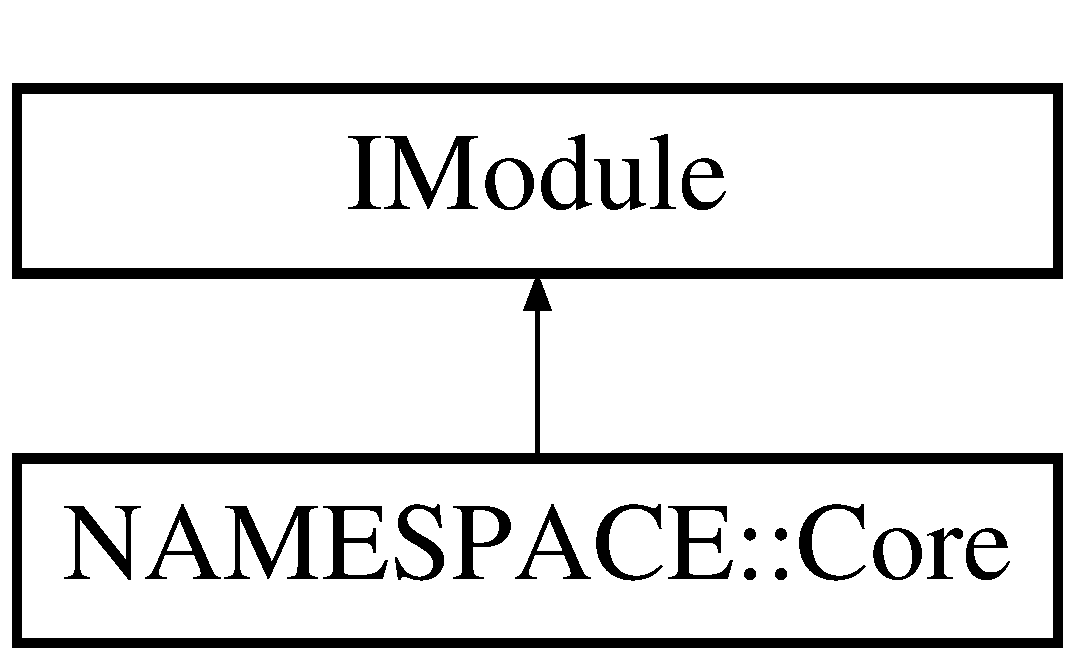
\includegraphics[height=2.000000cm]{class_n_a_m_e_s_p_a_c_e_1_1_core}
\end{center}
\end{figure}
\subsection*{Public Member Functions}
\begin{DoxyCompactItemize}
\item 
\hyperlink{class_n_a_m_e_s_p_a_c_e_1_1_core_a14e63188e0aa7c4a6f72d5501384d1f9}{Core} ()
\item 
\hyperlink{class_n_a_m_e_s_p_a_c_e_1_1_core_a5afb68389500c9f0537e852e486501b7}{Core} (const \hyperlink{class_n_a_m_e_s_p_a_c_e_1_1_core}{Core} \&rhs)
\item 
\hyperlink{class_n_a_m_e_s_p_a_c_e_1_1_core_a776f8c46504b14183883c6273f93eaed}{$\sim$\+Core} ()
\item 
double \hyperlink{class_n_a_m_e_s_p_a_c_e_1_1_core_a9aae5456022531811115080c388efdf4}{acceleration} (\hyperlink{class_n_a_m_e_s_p_a_c_e_1_1_agent}{Agent} $\ast$first, \hyperlink{class_n_a_m_e_s_p_a_c_e_1_1_agent}{Agent} $\ast$second)
\begin{DoxyCompactList}\small\item\em вычисляет необходимое ускорение \end{DoxyCompactList}\item 
void \hyperlink{class_n_a_m_e_s_p_a_c_e_1_1_core_a20d789ad96c8c29ec3568fd48bfe616b}{next\+\_\+step} ()
\end{DoxyCompactItemize}


\subsection{Detailed Description}
объект для обработки текущего состояния дорожной сцены 

... \begin{DoxyAuthor}{Author}
Серега 
\end{DoxyAuthor}
\begin{DoxyDate}{Date}
26.\+02.\+2017 
\end{DoxyDate}
\begin{DoxyVersion}{Version}
2 
\end{DoxyVersion}
\begin{DoxyRefDesc}{Bug}
\item[\hyperlink{bug__bug000001}{Bug}]... \end{DoxyRefDesc}
\begin{DoxyRefDesc}{Todo}
\item[\hyperlink{todo__todo000001}{Todo}]функция next\+\_\+step функциция spacing tbd константу \+\_\+alpha tbd константу \+\_\+delta tbd константу \+\_\+power \end{DoxyRefDesc}


\subsection{Constructor \& Destructor Documentation}
\mbox{\Hypertarget{class_n_a_m_e_s_p_a_c_e_1_1_core_a14e63188e0aa7c4a6f72d5501384d1f9}\label{class_n_a_m_e_s_p_a_c_e_1_1_core_a14e63188e0aa7c4a6f72d5501384d1f9}} 
\index{N\+A\+M\+E\+S\+P\+A\+C\+E\+::\+Core@{N\+A\+M\+E\+S\+P\+A\+C\+E\+::\+Core}!Core@{Core}}
\index{Core@{Core}!N\+A\+M\+E\+S\+P\+A\+C\+E\+::\+Core@{N\+A\+M\+E\+S\+P\+A\+C\+E\+::\+Core}}
\subsubsection{\texorpdfstring{Core()}{Core()}\hspace{0.1cm}{\footnotesize\ttfamily [1/2]}}
{\footnotesize\ttfamily Core\+::\+Core (\begin{DoxyParamCaption}{ }\end{DoxyParamCaption})}

\mbox{\Hypertarget{class_n_a_m_e_s_p_a_c_e_1_1_core_a5afb68389500c9f0537e852e486501b7}\label{class_n_a_m_e_s_p_a_c_e_1_1_core_a5afb68389500c9f0537e852e486501b7}} 
\index{N\+A\+M\+E\+S\+P\+A\+C\+E\+::\+Core@{N\+A\+M\+E\+S\+P\+A\+C\+E\+::\+Core}!Core@{Core}}
\index{Core@{Core}!N\+A\+M\+E\+S\+P\+A\+C\+E\+::\+Core@{N\+A\+M\+E\+S\+P\+A\+C\+E\+::\+Core}}
\subsubsection{\texorpdfstring{Core()}{Core()}\hspace{0.1cm}{\footnotesize\ttfamily [2/2]}}
{\footnotesize\ttfamily Core\+::\+Core (\begin{DoxyParamCaption}\item[{const \hyperlink{class_n_a_m_e_s_p_a_c_e_1_1_core}{Core} \&}]{rhs }\end{DoxyParamCaption})}

\mbox{\Hypertarget{class_n_a_m_e_s_p_a_c_e_1_1_core_a776f8c46504b14183883c6273f93eaed}\label{class_n_a_m_e_s_p_a_c_e_1_1_core_a776f8c46504b14183883c6273f93eaed}} 
\index{N\+A\+M\+E\+S\+P\+A\+C\+E\+::\+Core@{N\+A\+M\+E\+S\+P\+A\+C\+E\+::\+Core}!````~Core@{$\sim$\+Core}}
\index{````~Core@{$\sim$\+Core}!N\+A\+M\+E\+S\+P\+A\+C\+E\+::\+Core@{N\+A\+M\+E\+S\+P\+A\+C\+E\+::\+Core}}
\subsubsection{\texorpdfstring{$\sim$\+Core()}{~Core()}}
{\footnotesize\ttfamily Core\+::$\sim$\+Core (\begin{DoxyParamCaption}{ }\end{DoxyParamCaption})}



\subsection{Member Function Documentation}
\mbox{\Hypertarget{class_n_a_m_e_s_p_a_c_e_1_1_core_a9aae5456022531811115080c388efdf4}\label{class_n_a_m_e_s_p_a_c_e_1_1_core_a9aae5456022531811115080c388efdf4}} 
\index{N\+A\+M\+E\+S\+P\+A\+C\+E\+::\+Core@{N\+A\+M\+E\+S\+P\+A\+C\+E\+::\+Core}!acceleration@{acceleration}}
\index{acceleration@{acceleration}!N\+A\+M\+E\+S\+P\+A\+C\+E\+::\+Core@{N\+A\+M\+E\+S\+P\+A\+C\+E\+::\+Core}}
\subsubsection{\texorpdfstring{acceleration()}{acceleration()}}
{\footnotesize\ttfamily double Core\+::acceleration (\begin{DoxyParamCaption}\item[{\hyperlink{class_n_a_m_e_s_p_a_c_e_1_1_agent}{Agent} $\ast$}]{first,  }\item[{\hyperlink{class_n_a_m_e_s_p_a_c_e_1_1_agent}{Agent} $\ast$}]{second }\end{DoxyParamCaption})}



вычисляет необходимое ускорение 

вычисляет ускорение, необходимое агенту(first) для того, чтобы безопасно занять новое положение \begin{DoxyAuthor}{Author}
Серега 
\end{DoxyAuthor}
\begin{DoxyDate}{Date}
26.\+02.\+2017 
\end{DoxyDate}
\begin{DoxyVersion}{Version}
1 
\end{DoxyVersion}
\begin{DoxyRefDesc}{Bug}
\item[\hyperlink{bug__bug000002}{Bug}]... \end{DoxyRefDesc}
\begin{DoxyRefDesc}{Todo}
\item[\hyperlink{todo__todo000002}{Todo}]do this \end{DoxyRefDesc}
\mbox{\Hypertarget{class_n_a_m_e_s_p_a_c_e_1_1_core_a20d789ad96c8c29ec3568fd48bfe616b}\label{class_n_a_m_e_s_p_a_c_e_1_1_core_a20d789ad96c8c29ec3568fd48bfe616b}} 
\index{N\+A\+M\+E\+S\+P\+A\+C\+E\+::\+Core@{N\+A\+M\+E\+S\+P\+A\+C\+E\+::\+Core}!next\+\_\+step@{next\+\_\+step}}
\index{next\+\_\+step@{next\+\_\+step}!N\+A\+M\+E\+S\+P\+A\+C\+E\+::\+Core@{N\+A\+M\+E\+S\+P\+A\+C\+E\+::\+Core}}
\subsubsection{\texorpdfstring{next\+\_\+step()}{next\_step()}}
{\footnotesize\ttfamily void N\+A\+M\+E\+S\+P\+A\+C\+E\+::\+Core\+::next\+\_\+step (\begin{DoxyParamCaption}{ }\end{DoxyParamCaption})}

инкрементирует мдельное время

... \begin{DoxyAuthor}{Author}
Серега 
\end{DoxyAuthor}
\begin{DoxyDate}{Date}
26.\+02.\+2017 
\end{DoxyDate}
\begin{DoxyVersion}{Version}
0 
\end{DoxyVersion}
\begin{DoxyRefDesc}{Bug}
\item[\hyperlink{bug__bug000003}{Bug}]... \end{DoxyRefDesc}
\begin{DoxyRefDesc}{Todo}
\item[\hyperlink{todo__todo000003}{Todo}]do this \end{DoxyRefDesc}


The documentation for this class was generated from the following files\+:\begin{DoxyCompactItemize}
\item 
C\+R\+S/\+C\+R\+S/\hyperlink{core_8h}{core.\+h}\item 
C\+R\+S/\+C\+R\+S/\hyperlink{core_8cpp}{core.\+cpp}\end{DoxyCompactItemize}

\hypertarget{class_n_a_m_e_s_p_a_c_e_1_1_c_r_s}{}\section{N\+A\+M\+E\+S\+P\+A\+CE\+:\+:C\+RS Class Reference}
\label{class_n_a_m_e_s_p_a_c_e_1_1_c_r_s}\index{N\+A\+M\+E\+S\+P\+A\+C\+E\+::\+C\+RS@{N\+A\+M\+E\+S\+P\+A\+C\+E\+::\+C\+RS}}


{\ttfamily \#include $<$crs.\+h$>$}

Inheritance diagram for N\+A\+M\+E\+S\+P\+A\+CE\+:\+:C\+RS\+:\begin{figure}[H]
\begin{center}
\leavevmode
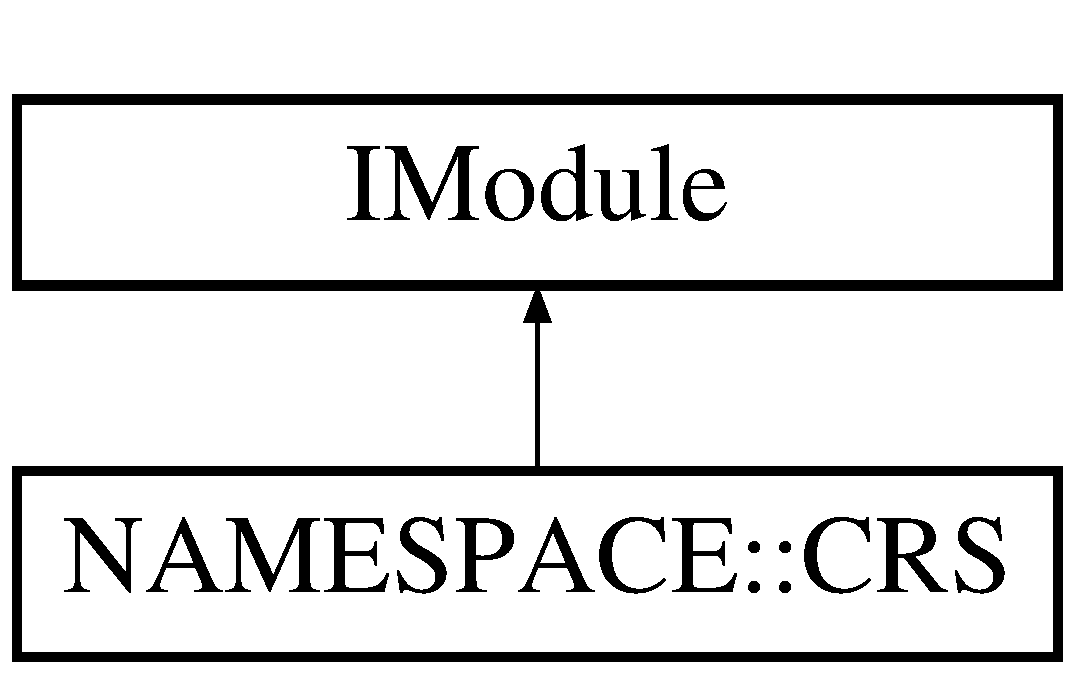
\includegraphics[height=2.000000cm]{class_n_a_m_e_s_p_a_c_e_1_1_c_r_s}
\end{center}
\end{figure}
\subsection*{Public Member Functions}
\begin{DoxyCompactItemize}
\item 
\hyperlink{class_n_a_m_e_s_p_a_c_e_1_1_c_r_s_a6d71ddf40c42ae57cacd47e6965cfe49}{C\+RS} ()
\item 
\hyperlink{class_n_a_m_e_s_p_a_c_e_1_1_c_r_s_a95dfa391c6ca4422f50fdc7d4ff7f895}{C\+RS} (const \hyperlink{class_n_a_m_e_s_p_a_c_e_1_1_c_r_s}{C\+RS} \&rhs)
\item 
\hyperlink{class_n_a_m_e_s_p_a_c_e_1_1_c_r_s_a994d4f0fa2a102a0c75ef813c0979c61}{$\sim$\+C\+RS} ()
\item 
\hyperlink{namespace_n_a_m_e_s_p_a_c_e_a610552ba0110b3ee573bc9f3a7a8eac4}{Agents} \hyperlink{class_n_a_m_e_s_p_a_c_e_1_1_c_r_s_ae81748dc264ab0f110a747fa78d9f570}{get\+\_\+agents} () const
\item 
\hyperlink{namespace_n_a_m_e_s_p_a_c_e_a610552ba0110b3ee573bc9f3a7a8eac4}{Agents} $\ast$ \hyperlink{class_n_a_m_e_s_p_a_c_e_1_1_c_r_s_ae352638954df2684ae3e080e99bb3d1b}{get\+\_\+access} ()
\item 
\hyperlink{class_n_a_m_e_s_p_a_c_e_1_1_agent}{Agent} $\ast$ \hyperlink{class_n_a_m_e_s_p_a_c_e_1_1_c_r_s_a1835af2e509fb495de3e5eb515fbd5cd}{get\+\_\+agent\+\_\+access} ()
\end{DoxyCompactItemize}


\subsection{Constructor \& Destructor Documentation}
\mbox{\Hypertarget{class_n_a_m_e_s_p_a_c_e_1_1_c_r_s_a6d71ddf40c42ae57cacd47e6965cfe49}\label{class_n_a_m_e_s_p_a_c_e_1_1_c_r_s_a6d71ddf40c42ae57cacd47e6965cfe49}} 
\index{N\+A\+M\+E\+S\+P\+A\+C\+E\+::\+C\+RS@{N\+A\+M\+E\+S\+P\+A\+C\+E\+::\+C\+RS}!C\+RS@{C\+RS}}
\index{C\+RS@{C\+RS}!N\+A\+M\+E\+S\+P\+A\+C\+E\+::\+C\+RS@{N\+A\+M\+E\+S\+P\+A\+C\+E\+::\+C\+RS}}
\subsubsection{\texorpdfstring{C\+R\+S()}{CRS()}\hspace{0.1cm}{\footnotesize\ttfamily [1/2]}}
{\footnotesize\ttfamily N\+A\+M\+E\+S\+P\+A\+C\+E\+::\+C\+R\+S\+::\+C\+RS (\begin{DoxyParamCaption}{ }\end{DoxyParamCaption})}

\mbox{\Hypertarget{class_n_a_m_e_s_p_a_c_e_1_1_c_r_s_a95dfa391c6ca4422f50fdc7d4ff7f895}\label{class_n_a_m_e_s_p_a_c_e_1_1_c_r_s_a95dfa391c6ca4422f50fdc7d4ff7f895}} 
\index{N\+A\+M\+E\+S\+P\+A\+C\+E\+::\+C\+RS@{N\+A\+M\+E\+S\+P\+A\+C\+E\+::\+C\+RS}!C\+RS@{C\+RS}}
\index{C\+RS@{C\+RS}!N\+A\+M\+E\+S\+P\+A\+C\+E\+::\+C\+RS@{N\+A\+M\+E\+S\+P\+A\+C\+E\+::\+C\+RS}}
\subsubsection{\texorpdfstring{C\+R\+S()}{CRS()}\hspace{0.1cm}{\footnotesize\ttfamily [2/2]}}
{\footnotesize\ttfamily N\+A\+M\+E\+S\+P\+A\+C\+E\+::\+C\+R\+S\+::\+C\+RS (\begin{DoxyParamCaption}\item[{const \hyperlink{class_n_a_m_e_s_p_a_c_e_1_1_c_r_s}{C\+RS} \&}]{rhs }\end{DoxyParamCaption})}

\mbox{\Hypertarget{class_n_a_m_e_s_p_a_c_e_1_1_c_r_s_a994d4f0fa2a102a0c75ef813c0979c61}\label{class_n_a_m_e_s_p_a_c_e_1_1_c_r_s_a994d4f0fa2a102a0c75ef813c0979c61}} 
\index{N\+A\+M\+E\+S\+P\+A\+C\+E\+::\+C\+RS@{N\+A\+M\+E\+S\+P\+A\+C\+E\+::\+C\+RS}!````~C\+RS@{$\sim$\+C\+RS}}
\index{````~C\+RS@{$\sim$\+C\+RS}!N\+A\+M\+E\+S\+P\+A\+C\+E\+::\+C\+RS@{N\+A\+M\+E\+S\+P\+A\+C\+E\+::\+C\+RS}}
\subsubsection{\texorpdfstring{$\sim$\+C\+R\+S()}{~CRS()}}
{\footnotesize\ttfamily N\+A\+M\+E\+S\+P\+A\+C\+E\+::\+C\+R\+S\+::$\sim$\+C\+RS (\begin{DoxyParamCaption}{ }\end{DoxyParamCaption})}



\subsection{Member Function Documentation}
\mbox{\Hypertarget{class_n_a_m_e_s_p_a_c_e_1_1_c_r_s_ae352638954df2684ae3e080e99bb3d1b}\label{class_n_a_m_e_s_p_a_c_e_1_1_c_r_s_ae352638954df2684ae3e080e99bb3d1b}} 
\index{N\+A\+M\+E\+S\+P\+A\+C\+E\+::\+C\+RS@{N\+A\+M\+E\+S\+P\+A\+C\+E\+::\+C\+RS}!get\+\_\+access@{get\+\_\+access}}
\index{get\+\_\+access@{get\+\_\+access}!N\+A\+M\+E\+S\+P\+A\+C\+E\+::\+C\+RS@{N\+A\+M\+E\+S\+P\+A\+C\+E\+::\+C\+RS}}
\subsubsection{\texorpdfstring{get\+\_\+access()}{get\_access()}}
{\footnotesize\ttfamily \hyperlink{namespace_n_a_m_e_s_p_a_c_e_a610552ba0110b3ee573bc9f3a7a8eac4}{Agents}$\ast$ N\+A\+M\+E\+S\+P\+A\+C\+E\+::\+C\+R\+S\+::get\+\_\+access (\begin{DoxyParamCaption}{ }\end{DoxyParamCaption})}

\mbox{\Hypertarget{class_n_a_m_e_s_p_a_c_e_1_1_c_r_s_a1835af2e509fb495de3e5eb515fbd5cd}\label{class_n_a_m_e_s_p_a_c_e_1_1_c_r_s_a1835af2e509fb495de3e5eb515fbd5cd}} 
\index{N\+A\+M\+E\+S\+P\+A\+C\+E\+::\+C\+RS@{N\+A\+M\+E\+S\+P\+A\+C\+E\+::\+C\+RS}!get\+\_\+agent\+\_\+access@{get\+\_\+agent\+\_\+access}}
\index{get\+\_\+agent\+\_\+access@{get\+\_\+agent\+\_\+access}!N\+A\+M\+E\+S\+P\+A\+C\+E\+::\+C\+RS@{N\+A\+M\+E\+S\+P\+A\+C\+E\+::\+C\+RS}}
\subsubsection{\texorpdfstring{get\+\_\+agent\+\_\+access()}{get\_agent\_access()}}
{\footnotesize\ttfamily \hyperlink{class_n_a_m_e_s_p_a_c_e_1_1_agent}{Agent}$\ast$ N\+A\+M\+E\+S\+P\+A\+C\+E\+::\+C\+R\+S\+::get\+\_\+agent\+\_\+access (\begin{DoxyParamCaption}{ }\end{DoxyParamCaption})}

\mbox{\Hypertarget{class_n_a_m_e_s_p_a_c_e_1_1_c_r_s_ae81748dc264ab0f110a747fa78d9f570}\label{class_n_a_m_e_s_p_a_c_e_1_1_c_r_s_ae81748dc264ab0f110a747fa78d9f570}} 
\index{N\+A\+M\+E\+S\+P\+A\+C\+E\+::\+C\+RS@{N\+A\+M\+E\+S\+P\+A\+C\+E\+::\+C\+RS}!get\+\_\+agents@{get\+\_\+agents}}
\index{get\+\_\+agents@{get\+\_\+agents}!N\+A\+M\+E\+S\+P\+A\+C\+E\+::\+C\+RS@{N\+A\+M\+E\+S\+P\+A\+C\+E\+::\+C\+RS}}
\subsubsection{\texorpdfstring{get\+\_\+agents()}{get\_agents()}}
{\footnotesize\ttfamily \hyperlink{namespace_n_a_m_e_s_p_a_c_e_a610552ba0110b3ee573bc9f3a7a8eac4}{Agents} N\+A\+M\+E\+S\+P\+A\+C\+E\+::\+C\+R\+S\+::get\+\_\+agents (\begin{DoxyParamCaption}{ }\end{DoxyParamCaption}) const}



The documentation for this class was generated from the following file\+:\begin{DoxyCompactItemize}
\item 
C\+R\+S/\+C\+R\+S/\hyperlink{crs_8h}{crs.\+h}\end{DoxyCompactItemize}

\hypertarget{class_i_module}{}\section{I\+Module Class Reference}
\label{class_i_module}\index{I\+Module@{I\+Module}}


{\ttfamily \#include $<$I\+Module.\+h$>$}

Inheritance diagram for I\+Module\+:\begin{figure}[H]
\begin{center}
\leavevmode
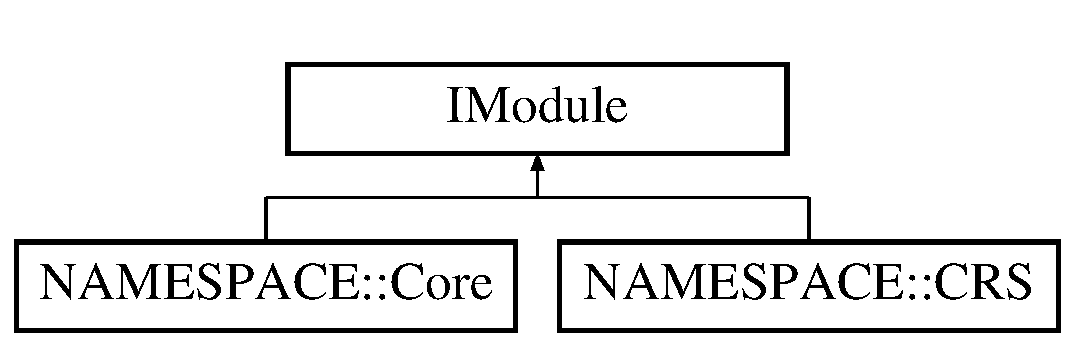
\includegraphics[height=2.000000cm]{class_i_module}
\end{center}
\end{figure}
\subsection*{Public Member Functions}
\begin{DoxyCompactItemize}
\item 
\hyperlink{class_i_module_ae926f787722b9aecd589be6c7aba1f66}{I\+Module} ()
\end{DoxyCompactItemize}


\subsection{Constructor \& Destructor Documentation}
\mbox{\Hypertarget{class_i_module_ae926f787722b9aecd589be6c7aba1f66}\label{class_i_module_ae926f787722b9aecd589be6c7aba1f66}} 
\index{I\+Module@{I\+Module}!I\+Module@{I\+Module}}
\index{I\+Module@{I\+Module}!I\+Module@{I\+Module}}
\subsubsection{\texorpdfstring{I\+Module()}{IModule()}}
{\footnotesize\ttfamily I\+Module\+::\+I\+Module (\begin{DoxyParamCaption}{ }\end{DoxyParamCaption})\hspace{0.3cm}{\ttfamily [inline]}}



The documentation for this class was generated from the following file\+:\begin{DoxyCompactItemize}
\item 
C\+R\+S/\+C\+R\+S/\hyperlink{_i_module_8h}{I\+Module.\+h}\end{DoxyCompactItemize}

\hypertarget{class_n_a_m_e_s_p_a_c_e_1_1_road}{}\section{N\+A\+M\+E\+S\+P\+A\+CE\+:\+:Road Class Reference}
\label{class_n_a_m_e_s_p_a_c_e_1_1_road}\index{N\+A\+M\+E\+S\+P\+A\+C\+E\+::\+Road@{N\+A\+M\+E\+S\+P\+A\+C\+E\+::\+Road}}


{\ttfamily \#include $<$Road.\+h$>$}

\subsection*{Public Member Functions}
\begin{DoxyCompactItemize}
\item 
\hyperlink{class_n_a_m_e_s_p_a_c_e_1_1_road_a98587c6f1f0ebc87b2dcab04c56a2cc7}{Road} ()
\item 
\hyperlink{class_n_a_m_e_s_p_a_c_e_1_1_road_af742f9e752a32eb16a62519b951bf1ae}{Road} (const \hyperlink{class_n_a_m_e_s_p_a_c_e_1_1_road}{Road} \&rhs)
\item 
\hyperlink{class_n_a_m_e_s_p_a_c_e_1_1_road_ab0c065a99eaa852463428b1744becffc}{$\sim$\+Road} ()
\end{DoxyCompactItemize}


\subsection{Constructor \& Destructor Documentation}
\mbox{\Hypertarget{class_n_a_m_e_s_p_a_c_e_1_1_road_a98587c6f1f0ebc87b2dcab04c56a2cc7}\label{class_n_a_m_e_s_p_a_c_e_1_1_road_a98587c6f1f0ebc87b2dcab04c56a2cc7}} 
\index{N\+A\+M\+E\+S\+P\+A\+C\+E\+::\+Road@{N\+A\+M\+E\+S\+P\+A\+C\+E\+::\+Road}!Road@{Road}}
\index{Road@{Road}!N\+A\+M\+E\+S\+P\+A\+C\+E\+::\+Road@{N\+A\+M\+E\+S\+P\+A\+C\+E\+::\+Road}}
\subsubsection{\texorpdfstring{Road()}{Road()}\hspace{0.1cm}{\footnotesize\ttfamily [1/2]}}
{\footnotesize\ttfamily N\+A\+M\+E\+S\+P\+A\+C\+E\+::\+Road\+::\+Road (\begin{DoxyParamCaption}{ }\end{DoxyParamCaption})}

\mbox{\Hypertarget{class_n_a_m_e_s_p_a_c_e_1_1_road_af742f9e752a32eb16a62519b951bf1ae}\label{class_n_a_m_e_s_p_a_c_e_1_1_road_af742f9e752a32eb16a62519b951bf1ae}} 
\index{N\+A\+M\+E\+S\+P\+A\+C\+E\+::\+Road@{N\+A\+M\+E\+S\+P\+A\+C\+E\+::\+Road}!Road@{Road}}
\index{Road@{Road}!N\+A\+M\+E\+S\+P\+A\+C\+E\+::\+Road@{N\+A\+M\+E\+S\+P\+A\+C\+E\+::\+Road}}
\subsubsection{\texorpdfstring{Road()}{Road()}\hspace{0.1cm}{\footnotesize\ttfamily [2/2]}}
{\footnotesize\ttfamily N\+A\+M\+E\+S\+P\+A\+C\+E\+::\+Road\+::\+Road (\begin{DoxyParamCaption}\item[{const \hyperlink{class_n_a_m_e_s_p_a_c_e_1_1_road}{Road} \&}]{rhs }\end{DoxyParamCaption})}

\mbox{\Hypertarget{class_n_a_m_e_s_p_a_c_e_1_1_road_ab0c065a99eaa852463428b1744becffc}\label{class_n_a_m_e_s_p_a_c_e_1_1_road_ab0c065a99eaa852463428b1744becffc}} 
\index{N\+A\+M\+E\+S\+P\+A\+C\+E\+::\+Road@{N\+A\+M\+E\+S\+P\+A\+C\+E\+::\+Road}!````~Road@{$\sim$\+Road}}
\index{````~Road@{$\sim$\+Road}!N\+A\+M\+E\+S\+P\+A\+C\+E\+::\+Road@{N\+A\+M\+E\+S\+P\+A\+C\+E\+::\+Road}}
\subsubsection{\texorpdfstring{$\sim$\+Road()}{~Road()}}
{\footnotesize\ttfamily N\+A\+M\+E\+S\+P\+A\+C\+E\+::\+Road\+::$\sim$\+Road (\begin{DoxyParamCaption}{ }\end{DoxyParamCaption})}



The documentation for this class was generated from the following file\+:\begin{DoxyCompactItemize}
\item 
C\+R\+S/\+C\+R\+S/\hyperlink{_road_8h}{Road.\+h}\end{DoxyCompactItemize}

\chapter{File Documentation}
\hypertarget{_agent_8h}{}\section{C\+R\+S/\+C\+R\+S/\+Agent.h File Reference}
\label{_agent_8h}\index{C\+R\+S/\+C\+R\+S/\+Agent.\+h@{C\+R\+S/\+C\+R\+S/\+Agent.\+h}}
{\ttfamily \#include \char`\"{}globaldefine.\+h\char`\"{}}\newline
{\ttfamily \#include \char`\"{}I\+Module.\+h\char`\"{}}\newline
{\ttfamily \#include $<$vector$>$}\newline
\subsection*{Classes}
\begin{DoxyCompactItemize}
\item 
class \hyperlink{class_n_a_m_e_s_p_a_c_e_1_1_agent}{N\+A\+M\+E\+S\+P\+A\+C\+E\+::\+Agent}
\begin{DoxyCompactList}\small\item\em объект отождествляющий собой участника движения(автомобиль) \end{DoxyCompactList}\end{DoxyCompactItemize}
\subsection*{Namespaces}
\begin{DoxyCompactItemize}
\item 
 \hyperlink{namespace_n_a_m_e_s_p_a_c_e}{N\+A\+M\+E\+S\+P\+A\+CE}
\end{DoxyCompactItemize}
\subsection*{Macros}
\begin{DoxyCompactItemize}
\item 
\#define \hyperlink{_agent_8h_a1f8ba4b0c4a03bec581e5d61c12aa576}{A\+G\+E\+N\+T\+\_\+H}
\end{DoxyCompactItemize}


\subsection{Macro Definition Documentation}
\mbox{\Hypertarget{_agent_8h_a1f8ba4b0c4a03bec581e5d61c12aa576}\label{_agent_8h_a1f8ba4b0c4a03bec581e5d61c12aa576}} 
\index{Agent.\+h@{Agent.\+h}!A\+G\+E\+N\+T\+\_\+H@{A\+G\+E\+N\+T\+\_\+H}}
\index{A\+G\+E\+N\+T\+\_\+H@{A\+G\+E\+N\+T\+\_\+H}!Agent.\+h@{Agent.\+h}}
\subsubsection{\texorpdfstring{A\+G\+E\+N\+T\+\_\+H}{AGENT\_H}}
{\footnotesize\ttfamily \#define A\+G\+E\+N\+T\+\_\+H}


\hypertarget{core_8cpp}{}\section{C\+R\+S/\+C\+R\+S/core.cpp File Reference}
\label{core_8cpp}\index{C\+R\+S/\+C\+R\+S/core.\+cpp@{C\+R\+S/\+C\+R\+S/core.\+cpp}}
{\ttfamily \#include \char`\"{}globaldefine.\+h\char`\"{}}\newline
{\ttfamily \#include \char`\"{}core.\+h\char`\"{}}\newline

\hypertarget{core_8h}{}\section{C\+R\+S/\+C\+R\+S/core.h File Reference}
\label{core_8h}\index{C\+R\+S/\+C\+R\+S/core.\+h@{C\+R\+S/\+C\+R\+S/core.\+h}}
{\ttfamily \#include \char`\"{}I\+Module.\+h\char`\"{}}\newline
{\ttfamily \#include \char`\"{}Agent.\+h\char`\"{}}\newline
\subsection*{Classes}
\begin{DoxyCompactItemize}
\item 
class \hyperlink{class_n_a_m_e_s_p_a_c_e_1_1_core}{N\+A\+M\+E\+S\+P\+A\+C\+E\+::\+Core}
\begin{DoxyCompactList}\small\item\em объект для обработки текущего состояния дорожной сцены \end{DoxyCompactList}\end{DoxyCompactItemize}
\subsection*{Namespaces}
\begin{DoxyCompactItemize}
\item 
 \hyperlink{namespace_n_a_m_e_s_p_a_c_e}{N\+A\+M\+E\+S\+P\+A\+CE}
\end{DoxyCompactItemize}
\subsection*{Macros}
\begin{DoxyCompactItemize}
\item 
\#define \hyperlink{core_8h_ae6acd7c0dd22c3e817d22221b2c84d7b}{C\+O\+R\+E\+\_\+H}
\end{DoxyCompactItemize}


\subsection{Macro Definition Documentation}
\mbox{\Hypertarget{core_8h_ae6acd7c0dd22c3e817d22221b2c84d7b}\label{core_8h_ae6acd7c0dd22c3e817d22221b2c84d7b}} 
\index{core.\+h@{core.\+h}!C\+O\+R\+E\+\_\+H@{C\+O\+R\+E\+\_\+H}}
\index{C\+O\+R\+E\+\_\+H@{C\+O\+R\+E\+\_\+H}!core.\+h@{core.\+h}}
\subsubsection{\texorpdfstring{C\+O\+R\+E\+\_\+H}{CORE\_H}}
{\footnotesize\ttfamily \#define C\+O\+R\+E\+\_\+H}


\hypertarget{crs_8h}{}\section{C\+R\+S/\+C\+R\+S/crs.h File Reference}
\label{crs_8h}\index{C\+R\+S/\+C\+R\+S/crs.\+h@{C\+R\+S/\+C\+R\+S/crs.\+h}}
{\ttfamily \#include \char`\"{}I\+Module.\+h\char`\"{}}\newline
{\ttfamily \#include $<$vector$>$}\newline
{\ttfamily \#include \char`\"{}Agent.\+h\char`\"{}}\newline
{\ttfamily \#include \char`\"{}Road.\+h\char`\"{}}\newline
\subsection*{Classes}
\begin{DoxyCompactItemize}
\item 
class \hyperlink{class_n_a_m_e_s_p_a_c_e_1_1_c_r_s}{N\+A\+M\+E\+S\+P\+A\+C\+E\+::\+C\+RS}
\end{DoxyCompactItemize}
\subsection*{Namespaces}
\begin{DoxyCompactItemize}
\item 
 \hyperlink{namespace_n_a_m_e_s_p_a_c_e}{N\+A\+M\+E\+S\+P\+A\+CE}
\end{DoxyCompactItemize}
\subsection*{Macros}
\begin{DoxyCompactItemize}
\item 
\#define \hyperlink{crs_8h_afb9f4a46a5b401e6749e0d717177a5b2}{C\+R\+S\+\_\+H}
\end{DoxyCompactItemize}
\subsection*{Typedefs}
\begin{DoxyCompactItemize}
\item 
typedef std\+::vector$<$ \hyperlink{class_n_a_m_e_s_p_a_c_e_1_1_agent}{Agent} $\ast$ $>$ \hyperlink{namespace_n_a_m_e_s_p_a_c_e_a610552ba0110b3ee573bc9f3a7a8eac4}{N\+A\+M\+E\+S\+P\+A\+C\+E\+::\+Agents}
\item 
typedef std\+::vector$<$ \hyperlink{class_n_a_m_e_s_p_a_c_e_1_1_road}{Road} $\ast$ $>$ \hyperlink{namespace_n_a_m_e_s_p_a_c_e_a2ec739fb2e81dc98134428bb29817671}{N\+A\+M\+E\+S\+P\+A\+C\+E\+::\+Roads}
\end{DoxyCompactItemize}


\subsection{Macro Definition Documentation}
\mbox{\Hypertarget{crs_8h_afb9f4a46a5b401e6749e0d717177a5b2}\label{crs_8h_afb9f4a46a5b401e6749e0d717177a5b2}} 
\index{crs.\+h@{crs.\+h}!C\+R\+S\+\_\+H@{C\+R\+S\+\_\+H}}
\index{C\+R\+S\+\_\+H@{C\+R\+S\+\_\+H}!crs.\+h@{crs.\+h}}
\subsubsection{\texorpdfstring{C\+R\+S\+\_\+H}{CRS\_H}}
{\footnotesize\ttfamily \#define C\+R\+S\+\_\+H}


\hypertarget{globaldefine_8h}{}\section{C\+R\+S/\+C\+R\+S/globaldefine.h File Reference}
\label{globaldefine_8h}\index{C\+R\+S/\+C\+R\+S/globaldefine.\+h@{C\+R\+S/\+C\+R\+S/globaldefine.\+h}}


файл содержит дефайны используемые во всем проекте  


\subsection*{Macros}
\begin{DoxyCompactItemize}
\item 
\#define \hyperlink{globaldefine_8h_afa7779fe56b160955b535cd6a8aaf8f4}{N\+A\+M\+E\+S\+P\+A\+CE}~C\+R\+S\+\_\+\+Project\+\_\+namespace
\end{DoxyCompactItemize}


\subsection{Detailed Description}
файл содержит дефайны используемые во всем проекте 

... \begin{DoxyAuthor}{Author}
Серега 
\end{DoxyAuthor}
\begin{DoxyDate}{Date}
19.\+02.\+2017 
\end{DoxyDate}
\begin{DoxyVersion}{Version}
1 
\end{DoxyVersion}
\begin{DoxyRefDesc}{Bug}
\item[\hyperlink{bug__bug000006}{Bug}]... \end{DoxyRefDesc}
\begin{DoxyRefDesc}{Todo}
\item[\hyperlink{todo__todo000006}{Todo}]... \end{DoxyRefDesc}


\subsection{Macro Definition Documentation}
\mbox{\Hypertarget{globaldefine_8h_afa7779fe56b160955b535cd6a8aaf8f4}\label{globaldefine_8h_afa7779fe56b160955b535cd6a8aaf8f4}} 
\index{globaldefine.\+h@{globaldefine.\+h}!N\+A\+M\+E\+S\+P\+A\+CE@{N\+A\+M\+E\+S\+P\+A\+CE}}
\index{N\+A\+M\+E\+S\+P\+A\+CE@{N\+A\+M\+E\+S\+P\+A\+CE}!globaldefine.\+h@{globaldefine.\+h}}
\subsubsection{\texorpdfstring{N\+A\+M\+E\+S\+P\+A\+CE}{NAMESPACE}}
{\footnotesize\ttfamily \#define N\+A\+M\+E\+S\+P\+A\+CE~C\+R\+S\+\_\+\+Project\+\_\+namespace}


\hypertarget{_i_module_8h}{}\section{C\+R\+S/\+C\+R\+S/\+I\+Module.h File Reference}
\label{_i_module_8h}\index{C\+R\+S/\+C\+R\+S/\+I\+Module.\+h@{C\+R\+S/\+C\+R\+S/\+I\+Module.\+h}}
{\ttfamily \#include $<$string$>$}\newline
\subsection*{Classes}
\begin{DoxyCompactItemize}
\item 
class \hyperlink{class_i_module}{I\+Module}
\end{DoxyCompactItemize}
\subsection*{Typedefs}
\begin{DoxyCompactItemize}
\item 
typedef int \hyperlink{_i_module_8h_af18a8a9ff181e7b64868286285ca6041}{S\+I\+G\+N\+A\+L\+\_\+\+T\+Y\+PE}
\item 
typedef int \hyperlink{_i_module_8h_a07da2e7fad77754487348ffa5f3aafd7}{T\+T\+O\+\_\+\+A\+PI}
\end{DoxyCompactItemize}


\subsection{Typedef Documentation}
\mbox{\Hypertarget{_i_module_8h_af18a8a9ff181e7b64868286285ca6041}\label{_i_module_8h_af18a8a9ff181e7b64868286285ca6041}} 
\index{I\+Module.\+h@{I\+Module.\+h}!S\+I\+G\+N\+A\+L\+\_\+\+T\+Y\+PE@{S\+I\+G\+N\+A\+L\+\_\+\+T\+Y\+PE}}
\index{S\+I\+G\+N\+A\+L\+\_\+\+T\+Y\+PE@{S\+I\+G\+N\+A\+L\+\_\+\+T\+Y\+PE}!I\+Module.\+h@{I\+Module.\+h}}
\subsubsection{\texorpdfstring{S\+I\+G\+N\+A\+L\+\_\+\+T\+Y\+PE}{SIGNAL\_TYPE}}
{\footnotesize\ttfamily typedef int \hyperlink{_i_module_8h_af18a8a9ff181e7b64868286285ca6041}{S\+I\+G\+N\+A\+L\+\_\+\+T\+Y\+PE}}

\mbox{\Hypertarget{_i_module_8h_a07da2e7fad77754487348ffa5f3aafd7}\label{_i_module_8h_a07da2e7fad77754487348ffa5f3aafd7}} 
\index{I\+Module.\+h@{I\+Module.\+h}!T\+T\+O\+\_\+\+A\+PI@{T\+T\+O\+\_\+\+A\+PI}}
\index{T\+T\+O\+\_\+\+A\+PI@{T\+T\+O\+\_\+\+A\+PI}!I\+Module.\+h@{I\+Module.\+h}}
\subsubsection{\texorpdfstring{T\+T\+O\+\_\+\+A\+PI}{TTO\_API}}
{\footnotesize\ttfamily typedef int \hyperlink{_i_module_8h_a07da2e7fad77754487348ffa5f3aafd7}{T\+T\+O\+\_\+\+A\+PI}}


\hypertarget{main_8cpp}{}\section{C\+R\+S/\+C\+R\+S/main.cpp File Reference}
\label{main_8cpp}\index{C\+R\+S/\+C\+R\+S/main.\+cpp@{C\+R\+S/\+C\+R\+S/main.\+cpp}}


основной файл проекта, запускает остальные модули  


{\ttfamily \#include \char`\"{}I\+Module.\+h\char`\"{}}\newline
{\ttfamily \#include $<$vector$>$}\newline
\subsection*{Typedefs}
\begin{DoxyCompactItemize}
\item 
typedef std\+::vector$<$ \hyperlink{class_i_module}{I\+Module} $\ast$ $>$ \hyperlink{main_8cpp_adeff7468f963b2e26f3f4c686f98fead}{Modules}
\end{DoxyCompactItemize}
\subsection*{Functions}
\begin{DoxyCompactItemize}
\item 
void \hyperlink{main_8cpp_ab68b0ca153dbee777accd1c361c55f89}{load} (\hyperlink{class_i_module}{I\+Module} $\ast$module)
\begin{DoxyCompactList}\small\item\em запускает исполняемые модули \end{DoxyCompactList}\item 
int \hyperlink{main_8cpp_a3c04138a5bfe5d72780bb7e82a18e627}{main} (int argc, char $\ast$$\ast$argv)
\begin{DoxyCompactList}\small\item\em основная функция проекта, точка входя программы \end{DoxyCompactList}\end{DoxyCompactItemize}


\subsection{Detailed Description}
основной файл проекта, запускает остальные модули 

... \begin{DoxyAuthor}{Author}
Серега 
\end{DoxyAuthor}
\begin{DoxyDate}{Date}
19.\+02.\+2017 
\end{DoxyDate}
\begin{DoxyVersion}{Version}
1 
\end{DoxyVersion}
\begin{DoxyRefDesc}{Bug}
\item[\hyperlink{bug__bug000007}{Bug}]... \end{DoxyRefDesc}
\begin{DoxyRefDesc}{Todo}
\item[\hyperlink{todo__todo000007}{Todo}]load function \end{DoxyRefDesc}


\subsection{Typedef Documentation}
\mbox{\Hypertarget{main_8cpp_adeff7468f963b2e26f3f4c686f98fead}\label{main_8cpp_adeff7468f963b2e26f3f4c686f98fead}} 
\index{main.\+cpp@{main.\+cpp}!Modules@{Modules}}
\index{Modules@{Modules}!main.\+cpp@{main.\+cpp}}
\subsubsection{\texorpdfstring{Modules}{Modules}}
{\footnotesize\ttfamily typedef std\+::vector$<$\hyperlink{class_i_module}{I\+Module}$\ast$$>$ \hyperlink{main_8cpp_adeff7468f963b2e26f3f4c686f98fead}{Modules}}



\subsection{Function Documentation}
\mbox{\Hypertarget{main_8cpp_ab68b0ca153dbee777accd1c361c55f89}\label{main_8cpp_ab68b0ca153dbee777accd1c361c55f89}} 
\index{main.\+cpp@{main.\+cpp}!load@{load}}
\index{load@{load}!main.\+cpp@{main.\+cpp}}
\subsubsection{\texorpdfstring{load()}{load()}}
{\footnotesize\ttfamily void load (\begin{DoxyParamCaption}\item[{\hyperlink{class_i_module}{I\+Module} $\ast$}]{module }\end{DoxyParamCaption})}



запускает исполняемые модули 

... \begin{DoxyAuthor}{Author}
Серега 
\end{DoxyAuthor}
\begin{DoxyDate}{Date}
19.\+02.\+2017 
\end{DoxyDate}
\begin{DoxyVersion}{Version}
1 
\end{DoxyVersion}
\begin{DoxyRefDesc}{Bug}
\item[\hyperlink{bug__bug000008}{Bug}]... \end{DoxyRefDesc}
\begin{DoxyRefDesc}{Todo}
\item[\hyperlink{todo__todo000008}{Todo}]do this \end{DoxyRefDesc}
\mbox{\Hypertarget{main_8cpp_a3c04138a5bfe5d72780bb7e82a18e627}\label{main_8cpp_a3c04138a5bfe5d72780bb7e82a18e627}} 
\index{main.\+cpp@{main.\+cpp}!main@{main}}
\index{main@{main}!main.\+cpp@{main.\+cpp}}
\subsubsection{\texorpdfstring{main()}{main()}}
{\footnotesize\ttfamily int main (\begin{DoxyParamCaption}\item[{int}]{argc,  }\item[{char $\ast$$\ast$}]{argv }\end{DoxyParamCaption})}



основная функция проекта, точка входя программы 

... \begin{DoxyAuthor}{Author}
Серега 
\end{DoxyAuthor}
\begin{DoxyDate}{Date}
19.\+02.\+2017 
\end{DoxyDate}
\begin{DoxyVersion}{Version}
1 
\end{DoxyVersion}
\begin{DoxyRefDesc}{Bug}
\item[\hyperlink{bug__bug000009}{Bug}]... \end{DoxyRefDesc}
\begin{DoxyRefDesc}{Todo}
\item[\hyperlink{todo__todo000009}{Todo}]... \end{DoxyRefDesc}

\hypertarget{_road_8h}{}\section{C\+R\+S/\+C\+R\+S/\+Road.h File Reference}
\label{_road_8h}\index{C\+R\+S/\+C\+R\+S/\+Road.\+h@{C\+R\+S/\+C\+R\+S/\+Road.\+h}}
\subsection*{Classes}
\begin{DoxyCompactItemize}
\item 
class \hyperlink{class_n_a_m_e_s_p_a_c_e_1_1_road}{N\+A\+M\+E\+S\+P\+A\+C\+E\+::\+Road}
\end{DoxyCompactItemize}
\subsection*{Namespaces}
\begin{DoxyCompactItemize}
\item 
 \hyperlink{namespace_n_a_m_e_s_p_a_c_e}{N\+A\+M\+E\+S\+P\+A\+CE}
\end{DoxyCompactItemize}

%--- End generated contents ---

% Index
\backmatter
\newpage
\phantomsection
\clearemptydoublepage
\addcontentsline{toc}{chapter}{Index}
\printindex

\end{document}
